\documentclass[11pt,letterpaper]{article}

\usepackage{graphicx}
\usepackage[margin=1in]{geometry}
\usepackage{amsmath}
\usepackage[T1]{fontenc}
\usepackage[utf8]{inputenc}
\usepackage{authblk}
\usepackage{fancyhdr}
\usepackage{lastpage}
\usepackage[parfill]{parskip}
\usepackage{subcaption}

\pagestyle{fancyplain}

% Headers
\lhead{}
\chead{}
\rhead{}

% Footers
\lfoot{}
\cfoot{}
\rfoot{\footnotesize Page \thepage\ of \pageref{LastPage}}

\renewcommand{\headrulewidth}{0.0pt} % No header rule
\renewcommand{\footrulewidth}{0.4pt} % Thin footer rule

\title{Federated Consistency Simulation: \\
 Realism Results with Conservative Tick Parameter}
\date{July 6, 2016}
\author[ ]{Benjamin Bengfort}
\author[ ]{Pete Keleher}
\affil[ ]{Department of Computer Science}
\affil[ ]{University of Maryland}
\affil[ ]{\textit{\{bengfort,keleher\}@cs.umd.edu}}

\begin{document}

\maketitle

\begin{abstract}
This report presents results from the federated consistency experiments using more realistic mean latencies and a conservative tick parameter (the so called Bailis model where $T=10\lambda_{\mu}$). The election timeout is $(T, 2T)$ and the heartbeat interval is $\frac{T} {2}$. The anti-entropy delay is $\frac {T} {4}$. The experiment includes all Raft, all Eventual, and Federated models run on 12 mean wide area latencies ($\lambda_{\mu}$) in the range 64ms -- 978ms with a $\lambda_{\sigma}=14$ for a total of 36 experiments (taking 1 hour 17 minutes to run 8 simulations in parallel at a time). These experiments were run on July 6, 2016 and include ``unforking'' -- Raft rejects writes that are forked by dropping them.
\end{abstract}

\begin{figure}[!h]
    \centering
        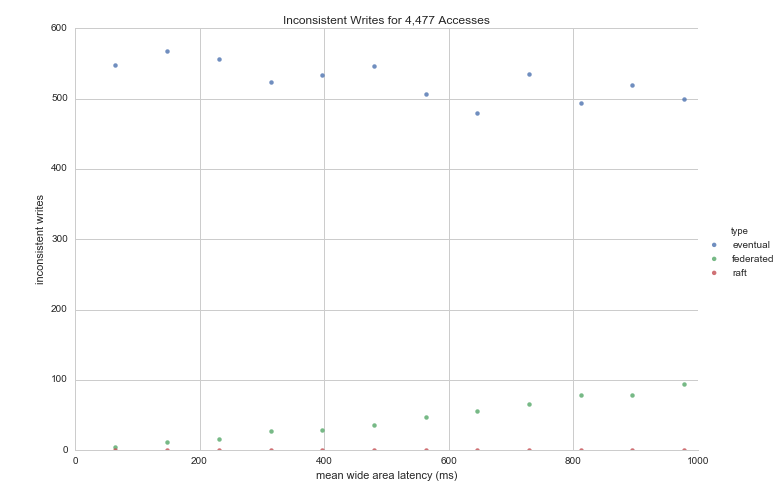
\includegraphics[width=\textwidth]{figures/inconsistent_writes.png}
        \caption{\textsf{Inconsistent writes are essentially forked writes less the number of writes that are dropped by Raft because they are forked. This figure shows the average number of conflicts in the system (the baseline) given by Eventual, and that Raft indeed has no inconsistent writes because it rejects forks. Federated consistency does have some insconsistent writes, those that occur on the Eventual side, but far less than Eventual by itself.}}
        \label{fig:inconsistent_writes}
\end{figure}

\begin{figure}[!h]
    \centering
        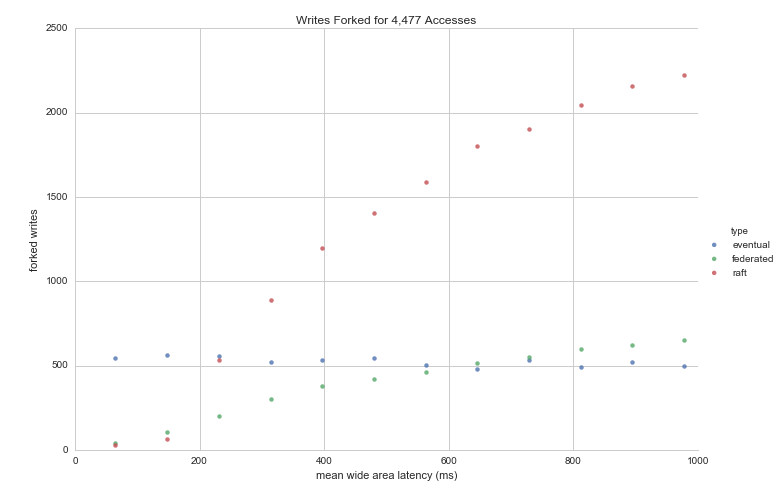
\includegraphics[width=\textwidth]{figures/forked_writes.png}
        \caption{\textsf{These are all of the forks that occur by writers in the system, again Eventual sets the baseline for the number of conflicts. Forks in Raft increase as the tick parameter increases because nodes are awaiting \texttt{AppendEntries} messages to write to in a \texttt{READ LATEST} fashion. All of these forks are simply dropped, as shown in Figure \ref{fig:dropped_writes}.}}
        \label{fig:forked_writes}
\end{figure}


\begin{figure}[!h]
    \centering
        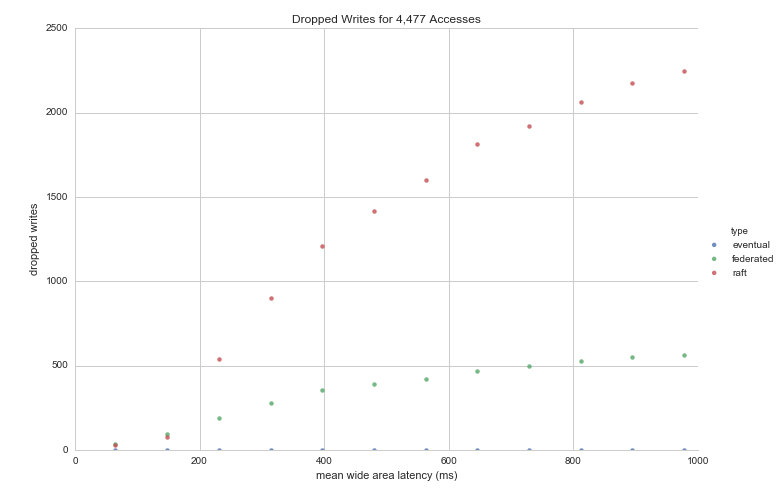
\includegraphics[width=\textwidth]{figures/dropped_writes.png}
        \caption{\textsf{The number of dropped writes are essentially write rejections, none of which occur in Eventual since the system is highly available. However, Raft must drop all inconsistent (e.g. forked) writes.}}
        \label{fig:dropped_writes}
\end{figure}

\begin{figure}[!h]
    \centering
        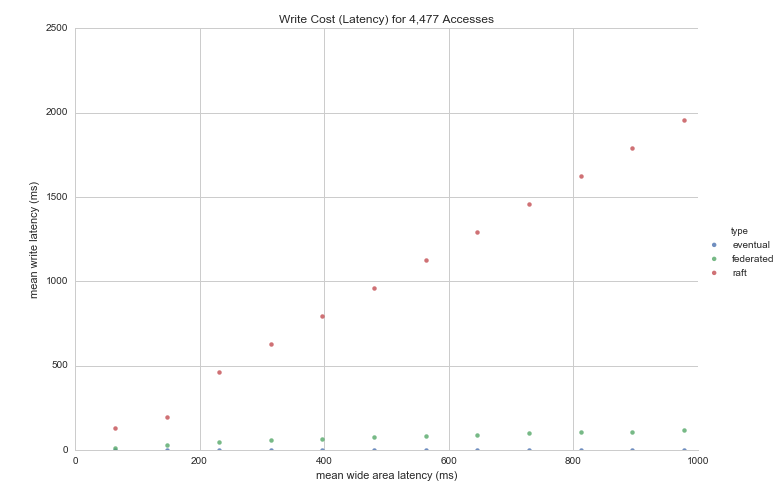
\includegraphics[width=\textwidth]{figures/write_latency.png}
        \caption{\textsf{As the mean wide area latency increases, so does the write cost in Raft since all Raft writes are remote writes. Federated takes on some of this cost, but also gains from the instantaneous writes in the eventual system, which has no write cost at all.}}
        \label{fig:write_latency}
\end{figure}


\begin{figure}[!h]
    \centering
        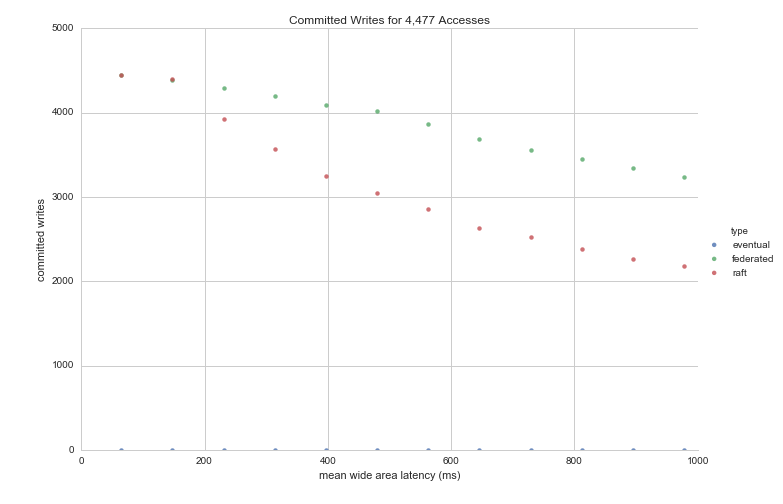
\includegraphics[width=\textwidth]{figures/committed_writes.png}
        \caption{\textsf{Eventual has no notion of commits, therefore there are zero commits in that system. Dropped writes are never committed. Therefore the difference between Federated and Raft here is that less writes are dropped and can thereby be committed, a drastic improvement!}}
        \label{fig:committed_writes}
\end{figure}

\begin{figure}[!h]
    \centering
        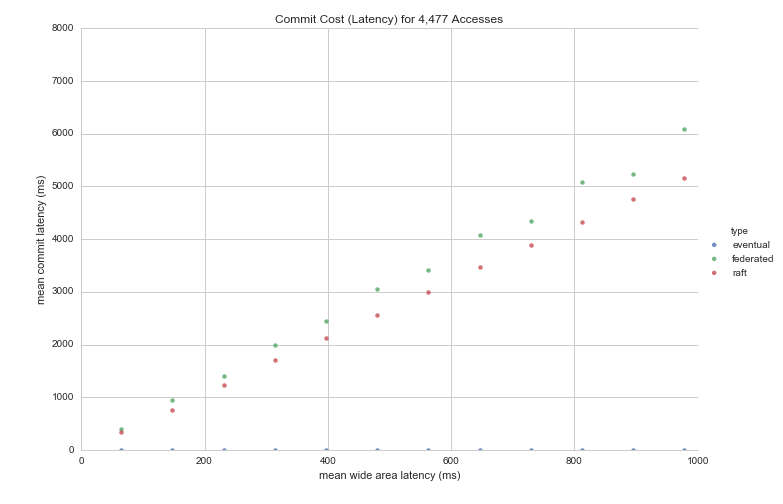
\includegraphics[width=\textwidth]{figures/commit_latency.png}
        \caption{\textsf{Both Raft and Federated experience a linear commit latency cost (two round trip \texttt{AppendEntries} for commit) as the mean wide area latency increases. Again, Eventual has no commit, therefore no commit latency.}}
        \label{fig:commit_latency}
\end{figure}

\begin{figure}[!h]
    \centering
        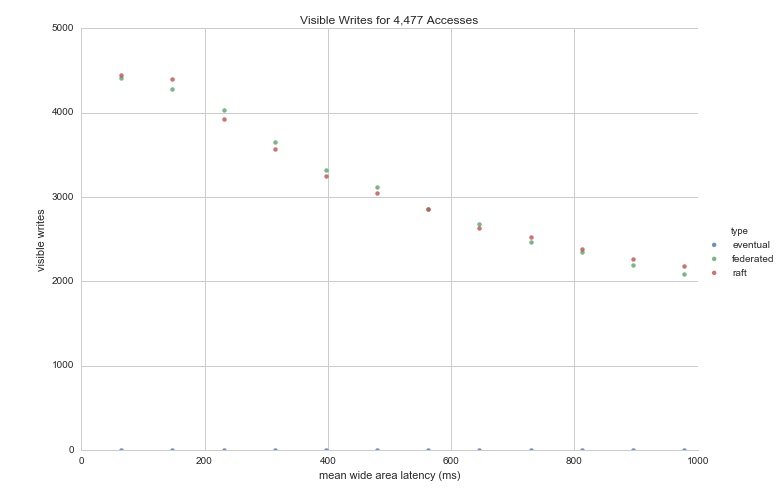
\includegraphics[width=\textwidth]{figures/visible_writes.png}
        \caption{\textsf{The number of writes that become visible, e.g. fully replicated. Raft and Federated have broadcast mechanisms that is able to transport the writes across the wide area much better than Eventual can. Note that dropped writes never become fully visible, hence the decrease in the fully visible percentage for Raft and Federated. That no writes become fully visible in Eventual is a product of both the anti-entropy delay and the write frequency which stomps writes before they can be replicated. Some work will have to be done to synchronize the entire log including previous writes.}}
        \label{fig:visible_writes}
\end{figure}

\begin{figure}[!h]
    \centering
        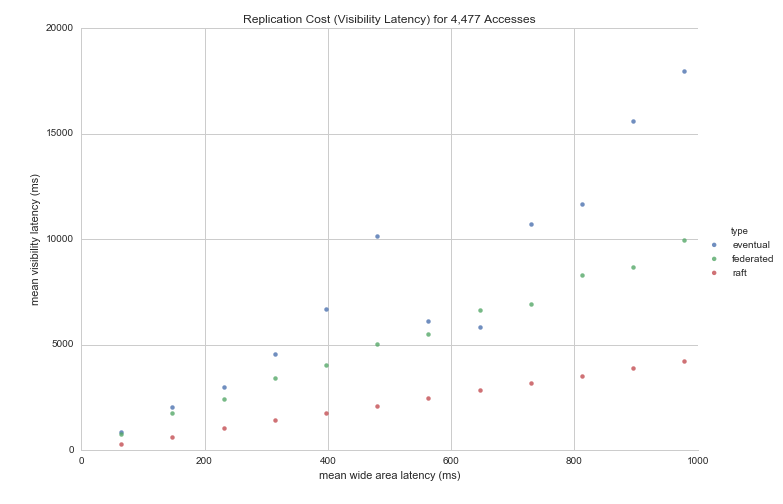
\includegraphics[width=\textwidth]{figures/visibility_latency.png}
        \caption{\textsf{The visibility latency is the time in ms it takes for a write to become fully visible. Raft does the best here since it is entirely one way broadcast from the leader to all other nodes in the system. Eventual does terrible since it relies on push based gossip to spread accesses across the network.}}
        \label{fig:visibility_latency}
\end{figure}

\begin{figure}[!h]
    \centering
        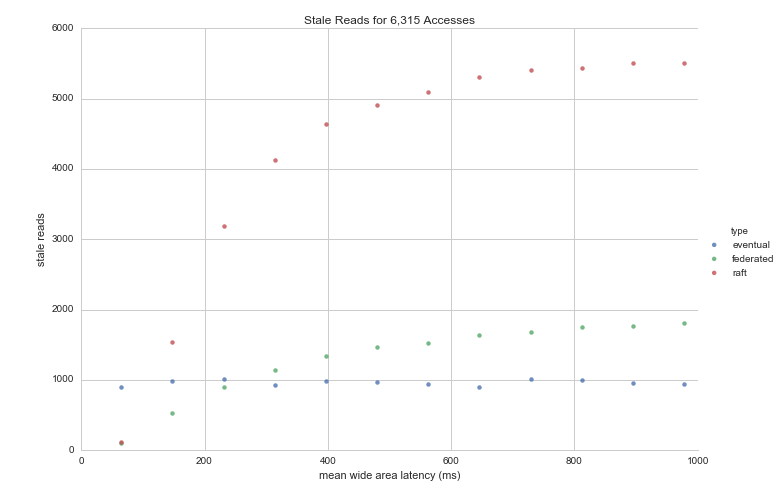
\includegraphics[width=\textwidth]{figures/stale_reads.png}
        \caption{\textsf{Eventual sets the baseline for the number of stale reads, both Federated and Raft are susceptible to stale reads where readers read locally the latest version but must wait \texttt{AppendEntries} for the latest version to show up. However, Federated's cross over point is much farther than Raft's. }}
        \label{fig:stale_reads}
\end{figure}

\begin{figure}[!h]
    \centering
        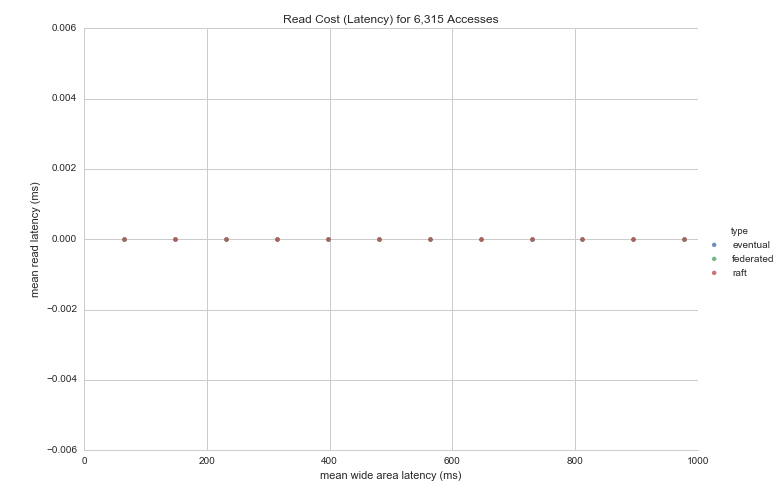
\includegraphics[width=\textwidth]{figures/read_latency.png}
        \caption{\textsf{There are no remote reads in this system, therefore read latency is instantaneous.}}
        \label{fig:read_latency}
\end{figure}

\begin{figure}[!h]
    \centering
        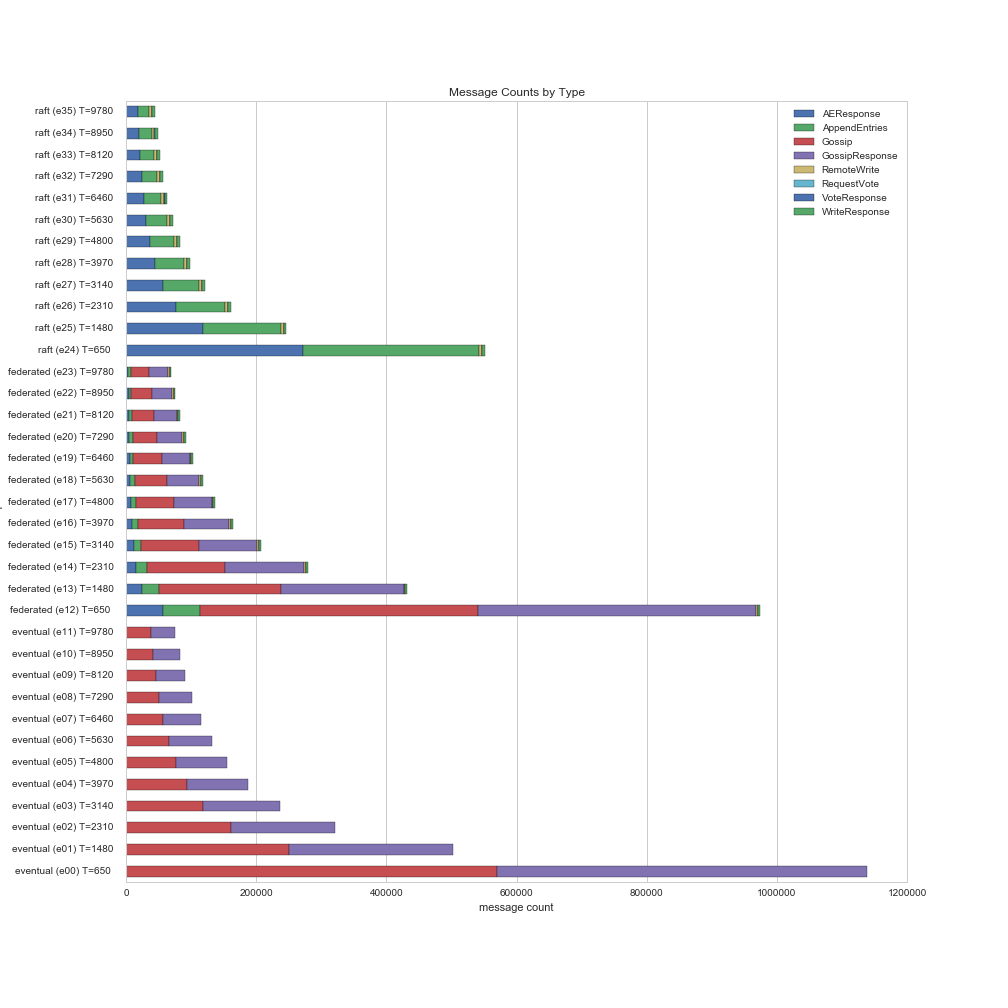
\includegraphics[width=\textwidth]{figures/message_counts.png}
        \caption{\textsf{The number of messages sent by a consistency model (either Raft or Eventual) is highly dependent on its timing parameters (election timeout, heartbeat interval, and anti-entropy delay). In our simulation we set our parameters according to a tick, T that is defined by the mean and standard deviation of the wide area latency.}}
        \label{fig:message_counts}
\end{figure}

\begin{figure}[!h]
    \centering
        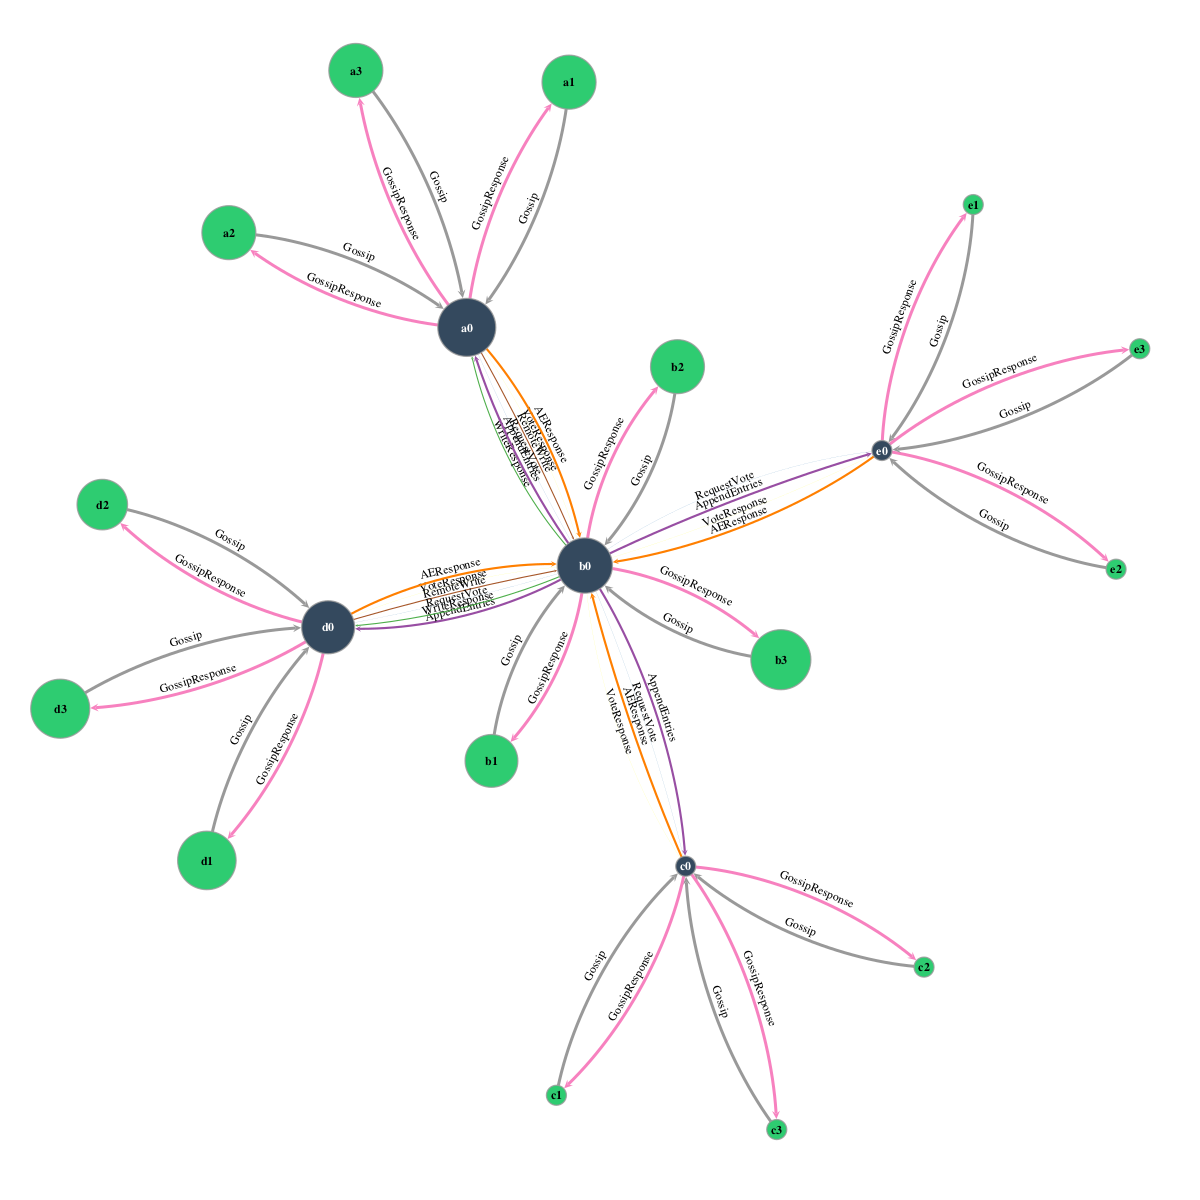
\includegraphics[width=\textwidth]{figures/federated-T1480.png}
        \caption{\textsf{Network topology of the federated consistency model. Edges define communication by message type (both color and label indicate the message type), message frequency between nodes is indicated by edge thickness. Vertices are colored by their consistency model (Raft and Eventual in Federated). Vertex size indicates the number of \textit{writes} that occurred at that node.}}
        \label{fig:topology}
\end{figure}

\begin{figure}[!h]
    \centering
        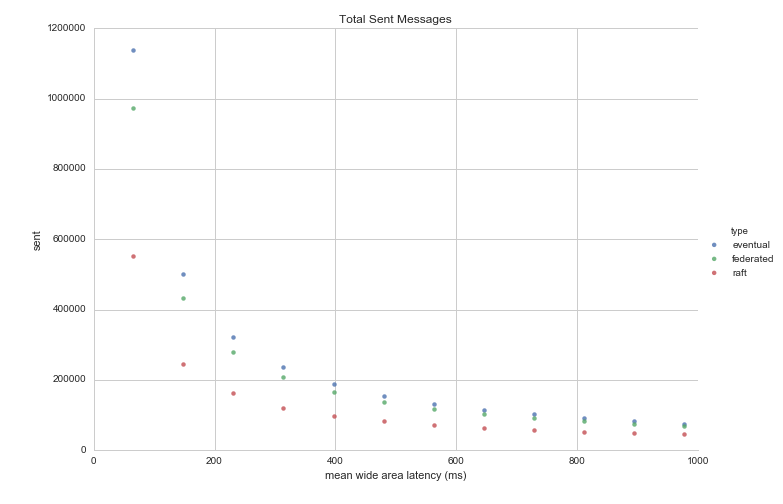
\includegraphics[width=\textwidth]{figures/messages_sent.png}
        \caption{\textsf{Total number of messages sent per consistency model. The lower the mean wide area latency, the lower the T, causing more messages to be sent. The number of messages is exponentially related to the mean network latency.}}
        \label{fig:messages_sent}
\end{figure}


\end{document}
